\section{\bfseries Slučajevi upotrebe}

\subsection{\bfseries Registrovanje i prijavljivanje korisnika}
\begin{figure}[H]
\begin{center}
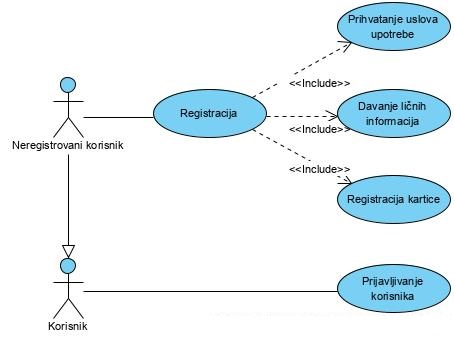
\includegraphics[scale=0.9]{Slike/UseCaseZaRegLog.jpg}
\end{center}
    \caption{Dijagram slučaja upotrebe registrovanja i prijavljivanja korisnika.}
\label{fig:RegistracijaPrijavljivanje}
\end{figure}


\subsubsection{\bfseries Registrovanje korisnika}

\begin{itemize}
    \item Kratak opis:
        \begin{itemize}
            \item Korisnik se kroz aplikaciju registruje kako bi mogao da koristi usluge CarGo.
        \end{itemize}
    \item Učesnici:
        \begin{itemize}
            \item Zainteresovana osoba koja želi da koristi usluge CarGo aplikacije.
        \end{itemize}
    \item Preduslovi:
        \begin{itemize}
            \item Korisnik mora da bude punoletan.
            \item Korisnik mora da bude državljanin Republike Srbije i da zna svoj JMBG.
            \item Korisnik mora da priloži tačne informacije pri registraciji.
            \item Korisnik mora da ima pametan telefon koji podržava aplikaciju.
            \item Korisnik mora da ima karticu za plaćanje koju može da registruje/koristi.
        \end{itemize}
    \item Postuslovi:
        \begin{itemize}
            \item Osoba je registrovana kao aktivni korisnik CarGo aplikacije.
        \end{itemize}
    \item Glavni tok:
        \begin{enumerate}
            \item Korisnik čita uslove korišćenja aplikacije pri pokretanju registracije.
            \item Korisnik prihvata postavljene uslove.
            \item Korisnik unosi lične podatke u vidu: mejl, korisničko ime, željena šifra.
            \item Korisnik unosi broj kartice kojom će vršiti plaćanje.
            \item Sistem omogućava korisniku prijavljivanje.
        \end{enumerate}
    \item Alternativni tok:
        \begin{itemize}
            \item Prilikom 2. koraka glavnog toka korisnik odbija uslove upotrebe aplikacije. Sistem obaveštava korisnika da mora da prihvati date uslove i onemogućava dalje korišćenje aplikacije dok se ne prihvate uslovi korišćenja.
            \item Prilikom koraka 4 glavnog toka korisnik preskače registraciju kartice pri čemu sistem onemogućava naručivanje vozila dok korisnik ne unese validan broj kartice.
        \end{itemize}
    \item Dodatne informacije:
        \begin{itemize}
            \item Uslovi upotrebe su regulisani zakonom. Nepoštovanje tih uslova može dovesti do ukidanja naloga korisnika i daljih sudskih postupaka.
        \end{itemize}
\end{itemize}

\begin{figure}[H]
\begin{center}
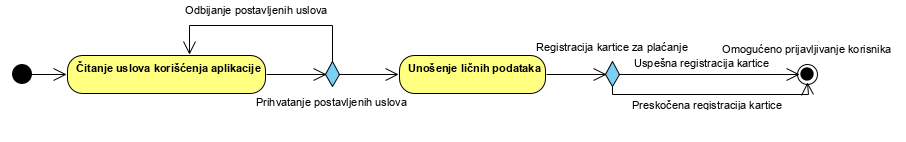
\includegraphics[width=\textwidth, height=125pt]{Slike/RegistracijaKorisnika.png}
\end{center}
    \caption{Dijagram aktivnosti registracije korisnika.}
\label{fig:RegistracijaKorisnika}
\end{figure}

\subsubsection{\bfseries Prijavljivanje korisnika}

\begin{itemize}
    \item Kratak opis:
        \begin{itemize}
            \item Korisnik koristi prethodno zapamćene informacije za prijavljivanje na aplikaciju.
        \end{itemize}
    \item Učesnici:
        \begin{itemize}
            \item Zainteresovana osoba koja želi da koristi usluge CarGo aplikacije.
        \end{itemize}
    \item Preduslovi:
        \begin{itemize}
            \item Korisnik mora da je registrovan da bi se uspešno prijavio
            \item Korisnik mora da zna svoje korisničko ime i šifru koju je koristio pri registraciji.
            \item Korisnik mora da ima pametan telefon koji podržava aplikaciju.
        \end{itemize}
    \item Postuslovi:
        \begin{itemize}
            \item Osoba je prijavljena kao aktivni korisnik i može da koristi aplikaciju.
        \end{itemize}
    \item Glavni tok:
        \begin{enumerate}
            \item Korisnik unosi svoje korisničko ime i šifru koju je koristio pri registraciji.
            \item Sistem proverava postojanje i tačnost podataka i prosleđuje korisnika dalje ka osnovnom interfejsu aplikacije.
        \end{enumerate}
    \item Alternativni tok:
        \begin{itemize}
            \item Ukoliko prilikom koraka 1 korisnik ne može da se seti svojih podataka, šalje mejl kontakt centru za pomoć. Sve dok korisnik ne unese podatke ostaje u koraku 1, a nakon unosa prelazi se na korak 2.
			\item Ukoliko korisnik ne unese validne podatke sistem ga obaveštava o greški prilikom prijavljivanja.
            \item Ukoliko korisnik u koraku 2 više puta ne uspe da se prijavi sa unetim podacima, dobija zabranu pokušaja 30 sekundi. Nakon tog perioda, korisnik je vraćen na korak 1.
        \end{itemize}
    \item Dodatne informacije:
        \begin{itemize}
            \item Zabrana prijavljivanja nakon nekoliko pokušaja obezbedjuje da CarGo server i korisnički podaci budu zaštićeni od 'brute force' napada.
        \end{itemize}
\end{itemize}


\subsection{\bfseries Rad sa vozačima}

\begin{figure}[H]
\begin{center}
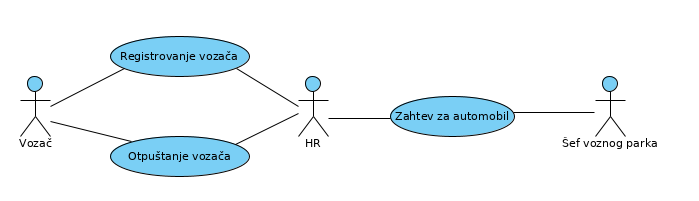
\includegraphics[width=\textwidth]{Slike/RadSaVozacimaUseCase.png}
\end{center}
    \caption{Slučajevi upotrebe Rad sa vozačima}
\label{fig:contextDiagram}
\end{figure}


\subsubsection{\bfseries Registrovanje vozača}

\begin{itemize}
	\item Kratak opis:
		\begin{itemize}
			\item Potencijalni vozač pristupa veb stranici i registruje se za pružanje usluga na putu.
		\end{itemize}
	\item Učesnici:
		\begin{itemize}
			\item Zainteresovana osoba koja želi da postane vozač CarGo zajendice.
		\end{itemize}				
	\item Preduslovi:
		\begin{itemize}
		    \item Prijavljeni mora da ima vozačku dozvolu.
		    \item Bar 5 godina iskustva u vožnji.
		    \item Napredno poznavanje grada.
		    \item Tehnički ispravan auto koji nije stariji od 10 godina ukoliko želi da koristi svoj lični auto. (U suprotnom će morati da prinese zahtev za dobijanje automobila za prevoz od strane CarGo zajednice)
		    \item Pametan telefon.
		    \item Uverenje da nije osuđivan.
		    \item Uspešno položen test ličnosti.
		\end{itemize}
	\item Postuslovi:
		\begin{itemize}
			\item Zainteresovana osoba je registrovana kao vozač.
		\end{itemize}		
	\item Glavni tok:
		\begin{enumerate}
		    \item Zainteresovana osoba pristupa veb stranici i nalazi formu za prijavu.
		    \item Zainteresovana osoba popunjava prijavu.
		    \item Na mejl stiže potvrda o uspešnosti prijavljivanja i termin dolaska na razgovor sa menadžerom za ljudske resurse.
		    \item Potencijalni vozač donosi na razgovor potrebnu dokumentaciju i radi test ličnosti.
		    \item Menadžer za ljudske resurse odlučuje da li je vozač kompetentan za tu poziciju i ukoliko jeste sistem beleži novog vozača u bazi.
		\end{enumerate}
	\item Alternativni tok:
		\begin{itemize}
    		\item Korak 2 - korisnik nije uneo ispravne podatke za prijavu. Slučaj upotrebe se nastavlja na drugom koraku glavnog toka.
		    \item Korak 4 - korisnik nije doneo potrebnu dokumentaciju na razgovor. U tom slučaju korisnik dobija novi termin za razgovor.
		\end{itemize}
	\item Dodatne informacije:
		\begin{itemize}
			\item Neophodni podaci za prijavu vozača su ime i prezime, validna e-mail adresa, broj telefona, godina registracije, marka i tip vozila pod uslovom da ima vozilo i za koji grad se prijavljuje.
		\end{itemize}						
\end{itemize}


\subsubsection{\bfseries Zahtev za automobil}

\begin{itemize}
	\item Kratak opis:
		\begin{itemize}
			\item Vozačima koji nemaju sopstveni automobil potrebno je obezbediti prevozno sredstvo.		
		\end{itemize}
	\item Učesnici:
		\begin{itemize}
		    \item Menadžer za ljudske resurse
		    \item Šef voznog parka
		    \item Vozač
		\end{itemize}
	\item Preduslovi:
		\begin{itemize}
		    \item Vozač je registrovan.
		    \item U prijavi je označeno da je potrebno vozilo.
		\end{itemize}
	\item Postuslovi:
		\begin{itemize}
			\item Vozač dobija vozilo.
	    \end{itemize}
	\item Glavni tok:
		\begin{enumerate}
		    \item Menadžer za ljudske resurse salje zahtev šefu voznog parka.
		    \item Šef voznog parka proverava da li ima slobodnih vozila.
		    \item Ukoliko ima dodeljuje slobodno vozilo vozaču.
		\end{enumerate}
	\item Alternativni tok:
		\begin{itemize}
		    \item Korak 2 - ukoliko nema slobodnih vozila, vozač se stavlja na čekanje i prelazi se na slucaj upotrebe nabavke vozila.
		\end{itemize}
	\item Dodatne informacije:
		\begin{itemize}
			\item Na osnovu prijave koju je dostavio vozač, menadžer za ljudske resurse zna da li on ima svoje vozilo ili je zatražio njihovo.
		\end{itemize}
\end{itemize}


\subsubsection{\bfseries Otpuštanje vozača}

\begin{itemize}
	\item Kratak opis:
		\begin{itemize}
			\item Prekid radnog odnosa sa vozačem.
		\end{itemize}
	\item Učesnici:
		\begin{itemize}
		    \item Menadžer za ljudske resurse
		    \item Vozač
		\end{itemize}
	\item Preduslovi:
		\begin{itemize}
		    \item Loša ocena.
		    \item Nezadovoljstvo radnika.
		    \item Nezadovoljstvo poslodavca.
		\end{itemize}
	\item Postuslovi:
		\begin{itemize}
			\item Vozač je otpušten.
	    \end{itemize}
	\item Glavni tok:
		\begin{enumerate}
		    \item Menadžer za ljudske resurse pokreće postupak otpuštanja vozača.
		    \item Vozač dobija otkaz.
		\end{enumerate}
	\item Alternativni tok:
		\begin{itemize}
		    \item Korak 2 - vozač svojevoljno podnosi zahtev za raskidanje radnog odnosa.
		\end{itemize}
\end{itemize}


\subsubsection{\bfseries Vraćanje vozila}

\begin{itemize}
	\item Kratak opis:
		\begin{itemize}
			\item Ukoliko vozač nije imao svoje vozilo i dobio je od firme, nakon prekida radnog odnosa vozač mora da vrati dobijeno vozilo šefu voznog parka.
		\end{itemize}
	\item Učesnici:
		\begin{itemize}
		    \item Vozač
		    \item Šef voznog parka
		\end{itemize}
	\item Preduslovi:
		\begin{itemize}
		    \item Vozač je otpušten.
		\end{itemize}
	\item Postuslovi:
		\begin{itemize}
			\item Vozilo je vraćeno.
	    \end{itemize}
	\item Glavni tok:
		\begin{enumerate}
		    \item Vozač daje ili dobija otkaz.
		    \item Vozač vraća vozilo.
		\end{enumerate}
\end{itemize}


\subsubsection{\bfseries Prijavljivanje vozača}

\begin{itemize}
    \item Kratak opis:
        \begin{itemize}
            \item Vozač koristi prethodno zapamćene informacije za prijavu na aplikaciju.
        \end{itemize}
    \item Učesnici:
        \begin{itemize}
            \item Vozač
        \end{itemize}
    \item Preduslovi:
        \begin{itemize}
            \item Vozač mora da zna svoje korisničko ime i šifru koju je koristio pri registraciji.
            \item Vozač mora da ima pametan telefon koji podržava aplikaciju.
        \end{itemize}
    \item Postuslovi:
        \begin{itemize}
            \item Vozač je prijavljen i može da koristi aplikaciju i vozi putnike.
        \end{itemize}
    \item Glavni tok:
        \begin{enumerate}
            \item Vozač unosi svoje korisničko ime i šifru koju je koristio pri registraciji.
            \item Sistem proverava postojanje i tačnost podataka i prosleđuje vozača dalje ka osnovnom interfejsu aplikacije.
        \end{enumerate}
    \item Alternativni tok:
        \begin{itemize}
            \item Korak 1 - vozač šalje mejl kontakt centru za pomoć ukoliko ne može da se seti svojih podataka.
            \item Korak 2 - uneti podaci nisu validni i sistem obaveštava korisnika o neuspešnom prijavljivanju.
            \item Korak 2 - ukoliko vozač više puta ne uspe da se prijavi sa unetim podacima, sistem postavlja zabranu pokušaja 30 sekundi. Nakon tog perioda, vozač je vraćen na korak 1.
        \end{itemize}
    \item Dodatne informacije:
        \begin{itemize}
            \item Zabrana prijavljivanja nakon nekoliko pokušaja obezbedjuje da CarGo server i korisnički podaci budu zaštićeni od 'brute force' napada.
        \end{itemize}
\end{itemize}

\subsection{\bfseries Vožnja}
\begin{figure}[H]
\begin{center}
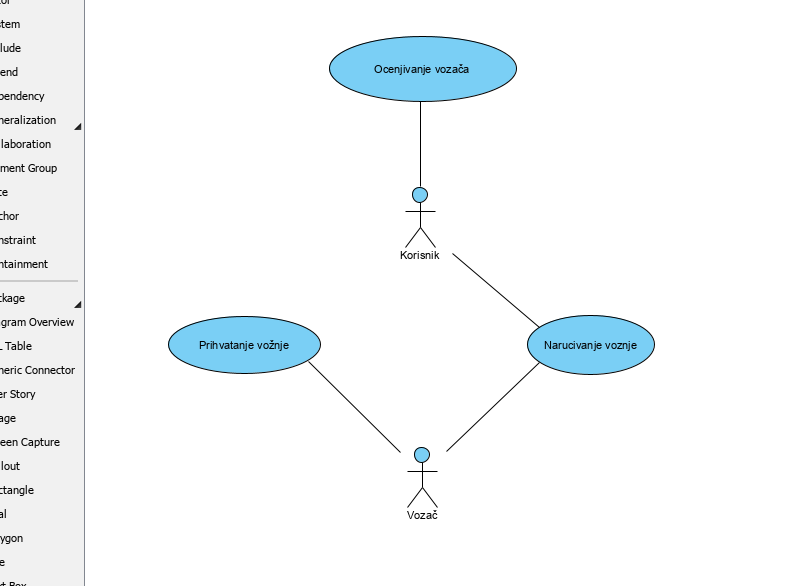
\includegraphics[scale=0.7]{Slike/VoznjaUseCase.png}
\end{center}
    \caption{Dijagram slučaja upotrebe Vožnja.}
\label{fig:Vožnja}
\end{figure}


\subsubsection{\bfseries Naručivanje vožnje}

\begin{itemize}
	\item Kratak opis:
		\begin{itemize}
			\item Korisnik naručuje vožnju radi transporta sa jednog odredišta na drugo.
		\end{itemize}
	\item Učesnici:
		\begin{itemize}
			\item Korisnik
		    \item Vozač
		\end{itemize}				
	\item Preduslovi:
		\begin{itemize}
		    \item Korisnik mora na svom telefonu posedovati aplikaciju.
		    \item Korisnik mora imati dovoljno novca na računu da bi mogao da plati vožnju.
		    \item Mora postojati slobodan vozač koji će moći da izvrši transport od jedne lokacije do druge.
		\end{itemize}
	\item Postuslovi:
		\begin{itemize}
			\item Vožnja je naručena.
		\end{itemize}		
	\item Glavni tok:
		\begin{enumerate}
		    \item Korisnik se prijavljuje na aplikaciju.
		    \item Definiše putem  aplikacije  početnu lokaciju.
		    \item Definiše lokaciju na koju želi da bude odvezen.
		    \item Zahtev se šalje serveru.
		    \item Server šalje zahtev vozačima.
		    \item Vozači koji žele i u mogućnosti su da prime vožnju to i čine.
		    \item Korisnik bira nekog od ponuđenih vozača u zavisnosti od nekoliko parametara (ocena vozača, udaljenost od trenutne lokacije, ukoliko mu cena odgovara).
		    \item Korisnik čeka odabranog vozača na definisanoj lokaciji u cilju transporta.
		\end{enumerate}
	\item Alternativni tok:
		\begin{itemize}
    		\item Korak 7 - ne postoji slobodno vozilo koje može izvršiti transport korisnika servisa ili koje zadovoljava želje korisnika. U tom slučaju korisnik se obaveštava da trenutno ne postoji slobodno vozilo i ukoliko to korisnik želi, stavlja se na listu čekanja dok se ne oslobodi neko vozilo.
		\end{itemize}
\end{itemize}


\subsubsection{\bfseries Prihvatanje vožnje}

\begin{itemize}
	\item Kratak opis:
		\begin{itemize}
			\item Vozač prihvata ili odbija zahtev za prevoz korisnika.
		\end{itemize}
	\item Učesnici:
		\begin{itemize}
		    \item Vozač
		\end{itemize}			
	\item Preduslovi:
		\begin{itemize}
		    \item Zahtev za prevoz poslat od strane korisnika.
		\end{itemize}
	\item Postuslovi:
		\begin{itemize}
			\item Vozač je prihvatio vožnju ukoliko je to želeo.
		\end{itemize}		
	\item Glavni tok:
		\begin{enumerate}
		    \item Korisnik šalje zahtev za prevoz.
		    \item Zahtev preko servera stiže do vozača.
		    \item Vozač prihvata ili odbija korisnički zahtev.
		\end{enumerate}
\end{itemize}


\subsubsection{\bfseries Prevoz putnika}

\begin{itemize}
	\item Kratak opis:
		\begin{itemize}
			\item Vrši se prevoz korisnika od strane vozača od jedne lokacije do druge.
		\end{itemize}
	\item Učesnici:
		\begin{itemize}
		    \item Korisnik
		    \item Vozač
		\end{itemize}				
	\item Preduslovi:
		\begin{itemize}
		    \item Korisnik mora da naruči vožnju.
		    \item Vozač mora da prihvati vožnju.
		    \item Korisnik mora da izabere jednog od vozača koji su prihvatili vožnju.
		\end{itemize}
	\item Postuslovi:
		\begin{itemize}
			\item Korisnik je stigao na željenu lokaciju.
		\end{itemize}	
	\item Glavni tok:
		\begin{enumerate}
		    \item Korisnik čeka da vozač stigne na prosleđenu lokaciju.
		    \item Vozač preuzima korisnika koji ga je unajmio.  
		    \item Vozač prevozi korisnika do ciljne lokacije.
		\end{enumerate}
\end{itemize}


\subsubsection{\bfseries Ocenjivanje vozača}

\begin{itemize}
	\item Kratak opis:
		\begin{itemize}
			\item Korisnik ocenjuje vozača na osnovu utisaka koji je isti na njega ostavio tokom vožnje.
		\end{itemize}
	\item Učesnici:
		\begin{itemize}
			\item Korisnik
		\end{itemize}				
	\item Preduslovi:
		\begin{itemize}
		    \item Korisnik prevežen od jedne lokacije do druge.
		\end{itemize}
	\item Postuslovi:
		\begin{itemize}
			\item Vozač je ocenjen ukoliko je korisnik želeo da ga oceni.
		\end{itemize}		
	\item Glavni tok:
		\begin{enumerate}
		    \item Korisnik prijavljuje putem aplikacije da je stigao na svoje odredište.
		    \item Korisnik bira da li hoće da oceni vozača.
		    \item Korisnik vrši ocenjivanje vozača ocenom od 1 do 5. 
		\end{enumerate}
	\item Alternativni tok:
		\begin{itemize}
		    \item Korak 1/2 - ukoliko je korisnik izuzetno nezadovoljan svojom vožnjom ili nije ni stigao na svoje odredište može da prijavi žalbu CarGo korisničkom servisu putem mejla ili CarGo web stranice.
    		\item Korak 2 - ukoliko je korisnik odabrao opciju da ne želi da oceni vozača korak 3 se preskače.
		\end{itemize}
\end{itemize}


\subsubsection{\bfseries Naplata vožnje}

\begin{itemize}
	\item Kratak opis:
		\begin{itemize}
			\item Korisnik isplaćuje uslugu prevoza.
		\end{itemize}
	\item Učesnici:
		\begin{itemize}
			\item Korisnik
			\item Banka
			\item Vozač
		\end{itemize}				
	\item Preduslovi:
		\begin{itemize}
		    \item Korisnik je prevežen do željene lokacije.
		\end{itemize}
	\item Postuslovi:
		\begin{itemize}
			\item Transakcija je uspešno obavljena.
		\end{itemize}		
	\item Glavni tok:
		\begin{enumerate}
		    \item Korisnik je stigao do željene lokacije.
		    \item Korisnik vrši uplatu novca (svota je definisana prilikom naručivanja vožnje) preko aplikacije.
		    \item Banka vrši prosleđivanje uplaćenog novca vozaču.
		    \item Vozaču leže uplata.
		\end{enumerate}
	\item Alternativni tok:
		\begin{itemize}
    		\item Korak 2 - korisnik plaća drugačiji iznos od unapred definisanog jer se može desiti da je ruta promenjena tokom vožnje (korisnik je zahtevao da se ide drugim putem) ili se krajnja lokacija ne poklapa sa onom koja je unapred definisana. Tok se nastavlja od koraka 3.
		\end{itemize}
\end{itemize}

\newpage

\subsection{\bfseries Nabavka vozila}

\begin{figure}[H]
\begin{center}
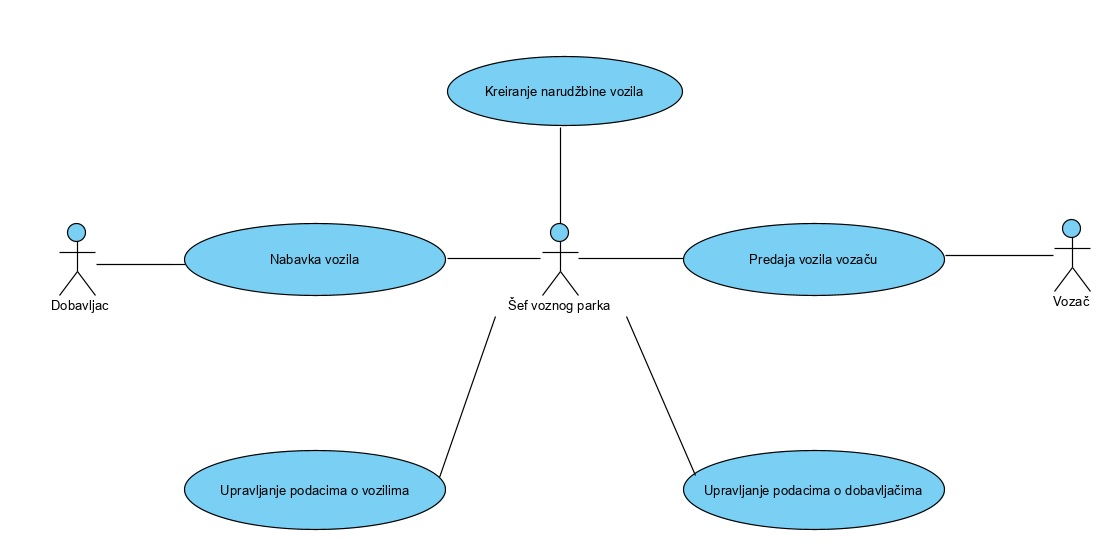
\includegraphics[width=\textwidth]{Slike/UseCaseZaVozniPark.jpg}
\end{center}
    \caption{Slučajevi upotrebe kod nabavke vozila.}
\label{fig:contextDiagram}
\end{figure}


\subsubsection{\bfseries Kreiranje narudžbine vozila}

\begin{itemize}
	\item Kratak opis:
		\begin{itemize}
			\item Šef voznog parka sastavlja porudžbinu o broju vozila pomoću informacije o vozačima kojima su potrebna vozila, a koju će kasnije proslediti dobavljaču vozila.
		\end{itemize}
	\item Učesnici:
		\begin{itemize}
		    \item Šef voznog parka
		\end{itemize}
	\item Preduslovi:
		\begin{itemize}
		    \item Postoje vozači kojima su potrebna vozila.
		\end{itemize}
	\item Postuslovi:
		\begin{itemize}
			\item Porudžbina je sastavljena i spremna za slanje.
	\end{itemize}
	\item Glavni tok:
		\begin{enumerate}
		    \item Šef voznog parka na nedeljnom nivou proverava bazu podataka o vozačima da bi video koliko novih vozača nema svoje vozilo.
		    \item Šef voznog parka proverava da li ima 10 ili više vozača kojima je potrebno vozilo ili postoji barem jedan vozač koji čeka na vozilo više od dve nedelje.
		    \item Šef voznog parka sastavlja porudžbinu.
		\end{enumerate}
	\item Alternativni tok:
		\begin{itemize}
		    \item Korak 2 - ukoliko ima manje od 10 vozača kojima je potrebno vozilo ili nijedan vozač ne čeka 2 nedelje, šef voznog parka čeka sledeću proveru baze o vozačima i kreće ponovo od koraka 2.
		\end{itemize}
\end{itemize}


\subsubsection{\bfseries Nabavka vozila}

\begin{itemize}
	\item Kratak opis:
		\begin{itemize}
			\item Šef voznog parka ima zadatak da naruči potrebnu količinu vozila kako bi ih prosledio novozaposlenim vozačima koji nemaju svoja vozila
		\end{itemize}
	\item Učesnici:
		\begin{itemize}
		    \item Šef voznog parka
			\item Dobavljač
		\end{itemize}
	\item Preduslovi:
		\begin{itemize}
		    \item Postoji barem jedan vozač koji nema svoje vozilo.
		\end{itemize}
	\item Postuslovi:
		\begin{itemize}
			\item Pribavljeno je onoliko vozila koliko ima vozača koji nemaju svoja ukoliko su ispunjeni uslovi
	\end{itemize}
	\item Glavni tok:
		\begin{enumerate}
		    \item Šef voznog parka proverava da li postoji neki vozač koji je zaposlen i nema svoje vozilo.
		    \item Šef voznog parka nakon provere sastavlja porudžbinu.
		    \item Šef voznog parka stupa u kontakt sa dobavljačem.
			\item Šef voznog parka isporučuje dobavljaču zahtevan broj vozila.
			\item Dobavljač prihvata porudžbinu.
			\item Dobavljač isporučuje šefu voznog parka zahtevan broj vozila.
			\item Šef voznog parka ih smešta u vozni park do raspodele vozila vozačima.
		\end{enumerate}
	\item Alternativni tok:
		\begin{itemize}
		    \item Korak 5 - u slučaju da dobavljač nije u stanju da ostvari porudžbinu, šef voznog parka odlaže nabavku u slučaju da su vozila potrebna za manje od 10 vozača ili pronalazi drugog dobavljača u slučaju da postoji 10 ili više vozača koji čekaju na vozila i nastavlja od koraka 5.
		\end{itemize}
\end{itemize}


\subsubsection{\bfseries Predaja vozila vozaču}

\begin{itemize}
	\item Kratak opis:
		\begin{itemize}
			\item Šef voznog parka prosleđuje vozilo iz voznog parka onom vozaču koji se zaposlio a nema svoje vozilo.
		\end{itemize}
	\item Učesnici:
		\begin{itemize}
		    \item Šef voznog parka
			\item Vozač
		\end{itemize}
	\item Preduslovi:
		\begin{itemize}
		    \item Vozač koji nema svoje vozilo pa čeka na vozilo firme.
		\end{itemize}
	\item Postuslovi:
		\begin{itemize}
			\item Vozaču je predato vozilo na korišćenje.
	\end{itemize}
	\item Glavni tok:
		\begin{enumerate}
		    \item Šef voznog parka obaveštava vozača da li ima vozilo.
		    \item Vozač i šef voznog parka se dogovaraju kada će se sastati.
		    \item Vozač i šef voznog parka se nalaze.
			\item Vozač napismeno prihvata odgovornost za to vozilo.
			\item Vozač preuzima vozilo.
		\end{enumerate}
	\item Alternativni tok:
		\begin{itemize}
		    \item Korak 1 - ukoliko šef voznog parka nema vozilo za vozača on dodaje vozača na spisak vozača koji čekaju na nabavku vozila nakon čega se kreće od koraka 1.
		\end{itemize}
\end{itemize}


\subsubsection{\bfseries Upravljanje podacima o vozačima}

\begin{itemize}
	\item Kratak opis:
		\begin{itemize}
			\item Šef voznog parka upravlja bazom podataka o vozilima pomoću operacija za čitanje i brisanje.
		\end{itemize}
	\item Učesnici:
		\begin{itemize}
		    \item Šef voznog parka
		\end{itemize}
	\item Preduslovi:
		\begin{itemize}
		    \item Baza podataka o vozačima je operativna.
		\end{itemize}
	\item Postuslovi:
		\begin{itemize}
			\item Šef voznog parka je ažurirao bazu podataka o vozačima.
	\end{itemize}
	\item Glavni tok:
		\begin{enumerate}
		    \item Šef voznog parka otvara program za rad sa bazom podataka o dobavljačima.
		    \item Šef voznog parka proverava da li ima barem 10 vozača koji nemaju svoja vozila.
		    \item Šef voznog parka kreira porudžbinu.
			\item Ažurira podatke u bazi o onim vozačima čija vozila će uključiti u porudžbinu.
		\end{enumerate}
	\item Alternativni tok:
		\begin{itemize}
		    \item Korak 1 - interfejs nije funkcionalan: Šef voznog parka mora da proba opet kasnije da pristupi bazi podataka.
			\item Korak 2 - ako nema 10 vozača ali postoji bar jedan vozač koji čeka na vozilo bar 2 nedelje: Šef voznog parka kreira porudžbinu za sve vozače koji čekaju na vozilo u tom momentu odnosno nastavlja od koraka 2.
		\end{itemize}
\end{itemize}


\subsubsection{\bfseries Upravljanje podacima o dobavljačima}

\begin{itemize}
	\item Kratak opis:
		\begin{itemize}
			\item Šef voznog parka upravlja bazom podataka o dobavljačima pomoću CRUD operacija.
		\end{itemize}
	\item Učesnici:
		\begin{itemize}
		    \item Šef voznog parka
		\end{itemize}
	\item Preduslovi:
		\begin{itemize}
		    \item Baza podataka o dobavljačima je operativna.
		\end{itemize}
	\item Postuslovi:
		\begin{itemize}
			\item Šef voznog parka je ažurirao bazu podataka o dobavljačima.
	    \end{itemize}
	\item Glavni tok:
		\begin{enumerate}
		    \item Šef voznog parka otvara interfejs za bazu podataka o dobavljačima.
		    \item Interfejs prikazuje trenutno stanje baze podataka.
		    \item Šef voznog parka bira operaciju koju želi da izvrši.
			\item Šef voznog parka izrvšava jednu od narednih operacija:
			\begin{itemize}
                \item Kreiranje:
                \begin{itemize}
                    \item Šef voznog parka unosi podatke o dobavljaču.
                    \item Šef voznog parka popunjava formu sa podacima o novom dobavljaču.
                    \item Šef voznog parka potvrđuje unos dobavljača u bazu podataka.
                \end{itemize}
                \item Čitanje:
                \begin{itemize}
                    \item Šef voznog parka pretražuje podatke o dobavljačima.
                    \item Šef voznog parka bira da vidi detaljne informacije o određenom dobavljaču.
                \end{itemize}
                \item Ažuriranje:
                \begin{itemize}
                    \item Šef voznog parka bira dobavljača čije informacije želi da ažurira.
                    \item Šef voznog parka prepravlja podatke o tom dobavljaču.
                    \item Šef voznog parka potvrđuje ažuriranje informacija o dobavljaču u bazi podataka.
                \end{itemize}
                \item Brisanje:
                \begin{itemize}
                    \item Šef voznog parka bira dobavljača kog želi da obriše.
                    \item Šef voznog parka briše odabranog dobavljača.
                    \item Šef voznog parka potvrđuje brisanje dobavljača iz baze podataka.
                \end{itemize}
            \end{itemize}
		\item Sistem pamti izmene u bazi podataka.
		\end{enumerate}
	\item Alternativni tok:
		\begin{itemize}
		    \item Korak 1 - interfejs nije funkcionalan: Šef voznog parka mora da proba opet kasnije da pristupi bazi podataka.
		\end{itemize}
\end{itemize}
